\documentclass[11pt,a4paper]{article}

% Essential packages
\usepackage[utf8]{inputenc}
\usepackage[T1]{fontenc}
\usepackage{lmodern}
\usepackage[english]{babel}

% Page layout
\usepackage[margin=2cm]{geometry}

% TikZ and related packages
\usepackage{tikz}
\usepackage{pgfplots}
\usepackage{tikz-cd}
\usepackage{circuitikz}
\usepackage{tikz-3dplot}

% TikZ libraries
\usetikzlibrary{
    arrows,
    arrows.meta,
    calc,
    decorations.markings,
    decorations.pathreplacing,
    fit,
    positioning,
    shapes,
    shapes.geometric,
    patterns,
    matrix,
    trees,
    backgrounds,
    shadows,
    plotmarks
}

% PGFPlots settings
\pgfplotsset{compat=1.18}

% Custom styles
% Common TikZ styles for consistent appearance
% Load this file in your main document with: % Common TikZ styles for consistent appearance
% Load this file in your main document with: % Common TikZ styles for consistent appearance
% Load this file in your main document with: \input{styles/common-styles.tex}

% Define common colors
\definecolor{primaryblue}{RGB}{52, 152, 219}
\definecolor{primaryred}{RGB}{231, 76, 60}
\definecolor{primarygreen}{RGB}{46, 204, 113}
\definecolor{primaryorange}{RGB}{230, 126, 34}
\definecolor{primarypurple}{RGB}{155, 89, 182}
\definecolor{lightgray}{RGB}{236, 240, 241}
\definecolor{darkgray}{RGB}{52, 73, 94}

% Node styles
\tikzset{
    % Basic node styles
    basic/.style={
        draw,
        rectangle,
        minimum width=2cm,
        minimum height=1cm,
        text centered,
        font=\footnotesize
    },
    % Process node
    process/.style={
        basic,
        fill=primaryblue!20,
        draw=primaryblue
    },
    % Decision node
    decision/.style={
        diamond,
        draw=primaryorange,
        fill=primaryorange!20,
        text width=1.5cm,
        text centered,
        font=\footnotesize
    },
    % Start/End node
    startstop/.style={
        basic,
        rounded corners=0.5cm,
        fill=primarygreen!20,
        draw=primarygreen
    },
    % Data node
    data/.style={
        basic,
        fill=primarypurple!20,
        draw=primarypurple
    },
    % Arrow styles
    arrow/.style={
        thick,
        ->,
        >=stealth
    },
    % Highlighted arrow
    highlight-arrow/.style={
        very thick,
        ->,
        >=stealth,
        color=primaryred
    },
    % Dotted arrow
    dotted-arrow/.style={
        thick,
        ->,
        >=stealth,
        dotted
    },
    % Axis styles
    axis/.style={
        thick,
        ->,
        >=stealth
    },
    % Grid style
    grid/.style={
        help lines,
        color=lightgray
    },
    % Function plot style
    plot/.style={
        thick,
        color=primaryblue,
        smooth
    },
    % Point style
    point/.style={
        circle,
        fill=primaryred,
        inner sep=2pt
    }
}


% Define common colors
\definecolor{primaryblue}{RGB}{52, 152, 219}
\definecolor{primaryred}{RGB}{231, 76, 60}
\definecolor{primarygreen}{RGB}{46, 204, 113}
\definecolor{primaryorange}{RGB}{230, 126, 34}
\definecolor{primarypurple}{RGB}{155, 89, 182}
\definecolor{lightgray}{RGB}{236, 240, 241}
\definecolor{darkgray}{RGB}{52, 73, 94}

% Node styles
\tikzset{
    % Basic node styles
    basic/.style={
        draw,
        rectangle,
        minimum width=2cm,
        minimum height=1cm,
        text centered,
        font=\footnotesize
    },
    % Process node
    process/.style={
        basic,
        fill=primaryblue!20,
        draw=primaryblue
    },
    % Decision node
    decision/.style={
        diamond,
        draw=primaryorange,
        fill=primaryorange!20,
        text width=1.5cm,
        text centered,
        font=\footnotesize
    },
    % Start/End node
    startstop/.style={
        basic,
        rounded corners=0.5cm,
        fill=primarygreen!20,
        draw=primarygreen
    },
    % Data node
    data/.style={
        basic,
        fill=primarypurple!20,
        draw=primarypurple
    },
    % Arrow styles
    arrow/.style={
        thick,
        ->,
        >=stealth
    },
    % Highlighted arrow
    highlight-arrow/.style={
        very thick,
        ->,
        >=stealth,
        color=primaryred
    },
    % Dotted arrow
    dotted-arrow/.style={
        thick,
        ->,
        >=stealth,
        dotted
    },
    % Axis styles
    axis/.style={
        thick,
        ->,
        >=stealth
    },
    % Grid style
    grid/.style={
        help lines,
        color=lightgray
    },
    % Function plot style
    plot/.style={
        thick,
        color=primaryblue,
        smooth
    },
    % Point style
    point/.style={
        circle,
        fill=primaryred,
        inner sep=2pt
    }
}


% Define common colors
\definecolor{primaryblue}{RGB}{52, 152, 219}
\definecolor{primaryred}{RGB}{231, 76, 60}
\definecolor{primarygreen}{RGB}{46, 204, 113}
\definecolor{primaryorange}{RGB}{230, 126, 34}
\definecolor{primarypurple}{RGB}{155, 89, 182}
\definecolor{lightgray}{RGB}{236, 240, 241}
\definecolor{darkgray}{RGB}{52, 73, 94}

% Node styles
\tikzset{
    % Basic node styles
    basic/.style={
        draw,
        rectangle,
        minimum width=2cm,
        minimum height=1cm,
        text centered,
        font=\footnotesize
    },
    % Process node
    process/.style={
        basic,
        fill=primaryblue!20,
        draw=primaryblue
    },
    % Decision node
    decision/.style={
        diamond,
        draw=primaryorange,
        fill=primaryorange!20,
        text width=1.5cm,
        text centered,
        font=\footnotesize
    },
    % Start/End node
    startstop/.style={
        basic,
        rounded corners=0.5cm,
        fill=primarygreen!20,
        draw=primarygreen
    },
    % Data node
    data/.style={
        basic,
        fill=primarypurple!20,
        draw=primarypurple
    },
    % Arrow styles
    arrow/.style={
        thick,
        ->,
        >=stealth
    },
    % Highlighted arrow
    highlight-arrow/.style={
        very thick,
        ->,
        >=stealth,
        color=primaryred
    },
    % Dotted arrow
    dotted-arrow/.style={
        thick,
        ->,
        >=stealth,
        dotted
    },
    % Axis styles
    axis/.style={
        thick,
        ->,
        >=stealth
    },
    % Grid style
    grid/.style={
        help lines,
        color=lightgray
    },
    % Function plot style
    plot/.style={
        thick,
        color=primaryblue,
        smooth
    },
    % Point style
    point/.style={
        circle,
        fill=primaryred,
        inner sep=2pt
    }
}


% Document information
\title{TikZ Graphics Collection}
\author{Your Name}
\date{\today}

\begin{document}

\maketitle

\section{Complete Graph K4}

This document contains a complete graph with 4 nodes (A, B, C, D) where every node is connected to every other node.

\begin{figure}[h]
    \centering
    \resizebox{\textwidth}{!}{\input{tikz/figures/example_graph.tex}}
    \caption{Complete Graph K4 with nodes A, B, C, and D}
    \label{fig:complete-graph-k4}
\end{figure}

\section{GNN Architecture for Road Networks}

This diagram illustrates the flow from a road network graph through a Graph Neural Network (GNN) layer to produce a city embedding vector.

\begin{figure}[h]
    \centering
    % GNN Architecture Diagram
% Shows graph input -> GNN layer -> city embedding vector

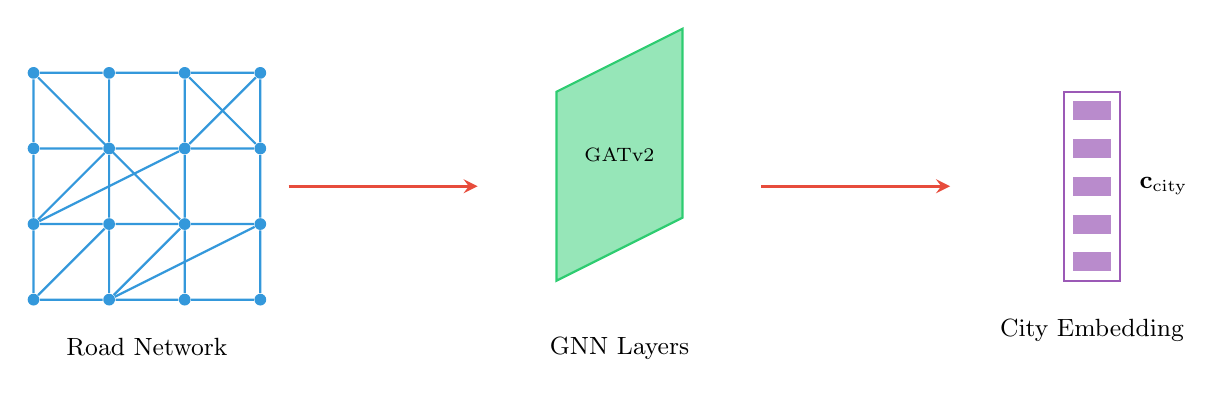
\begin{tikzpicture}[scale=1.2]
    
    % Define coordinates
    \coordinate (graph-center) at (0,0);
    \coordinate (gnn-center) at (5,0);
    \coordinate (vector-pos) at (10,0);
    
    % Draw road network graph on the left
    \begin{scope}[shift={(graph-center)}]
        % Create a grid-like road network with intersections
        % Define nodes manually to avoid decimal naming issues
        \node[circle, fill=primaryblue, inner sep=1.5pt] (n11) at (-1.2, -1.2) {};
        \node[circle, fill=primaryblue, inner sep=1.5pt] (n12) at (-1.2, -0.4) {};
        \node[circle, fill=primaryblue, inner sep=1.5pt] (n13) at (-1.2, 0.4) {};
        \node[circle, fill=primaryblue, inner sep=1.5pt] (n14) at (-1.2, 1.2) {};
        
        \node[circle, fill=primaryblue, inner sep=1.5pt] (n21) at (-0.4, -1.2) {};
        \node[circle, fill=primaryblue, inner sep=1.5pt] (n22) at (-0.4, -0.4) {};
        \node[circle, fill=primaryblue, inner sep=1.5pt] (n23) at (-0.4, 0.4) {};
        \node[circle, fill=primaryblue, inner sep=1.5pt] (n24) at (-0.4, 1.2) {};
        
        \node[circle, fill=primaryblue, inner sep=1.5pt] (n31) at (0.4, -1.2) {};
        \node[circle, fill=primaryblue, inner sep=1.5pt] (n32) at (0.4, -0.4) {};
        \node[circle, fill=primaryblue, inner sep=1.5pt] (n33) at (0.4, 0.4) {};
        \node[circle, fill=primaryblue, inner sep=1.5pt] (n34) at (0.4, 1.2) {};
        
        \node[circle, fill=primaryblue, inner sep=1.5pt] (n41) at (1.2, -1.2) {};
        \node[circle, fill=primaryblue, inner sep=1.5pt] (n42) at (1.2, -0.4) {};
        \node[circle, fill=primaryblue, inner sep=1.5pt] (n43) at (1.2, 0.4) {};
        \node[circle, fill=primaryblue, inner sep=1.5pt] (n44) at (1.2, 1.2) {};
        
        % Horizontal road connections
        \draw[thick, primaryblue] (n11) -- (n21) -- (n31) -- (n41);
        \draw[thick, primaryblue] (n12) -- (n22) -- (n32) -- (n42);
        \draw[thick, primaryblue] (n13) -- (n23) -- (n33) -- (n43);
        \draw[thick, primaryblue] (n14) -- (n24) -- (n34) -- (n44);
        
        % Vertical road connections
        \draw[thick, primaryblue] (n11) -- (n12) -- (n13) -- (n14);
        \draw[thick, primaryblue] (n21) -- (n22) -- (n23) -- (n24);
        \draw[thick, primaryblue] (n31) -- (n32) -- (n33) -- (n34);
        \draw[thick, primaryblue] (n41) -- (n42) -- (n43) -- (n44);
        
        % Add some diagonal connections to make it more realistic
        \draw[thick, primaryblue] (n11) -- (n22);
        \draw[thick, primaryblue] (n33) -- (n44);
        \draw[thick, primaryblue] (n21) -- (n32);
        \draw[thick, primaryblue] (n12) -- (n23);
        \draw[thick, primaryblue] (n34) -- (n43);
        
        % Add some additional random connections to simulate non-grid roads
        \draw[thick, primaryblue] (n12) -- (n33);
        \draw[thick, primaryblue] (n21) -- (n42);
        \draw[thick, primaryblue] (n14) -- (n32);
        
        % Graph label
        \node[below] at (0, -1.5) {\small Road Network};
    \end{scope}
    
    % Arrow from graph to GNN
    \draw[arrow, very thick, primaryred] (1.5, 0) -- (3.5, 0);
    
        % GNN layer as stacked parallelogram blocks in perspective
    \begin{scope}[shift={(gnn-center)}]
        % Parameters for parallelograms
        \def\w{4 / 3}   % width
        \def\h{2}   % height
        \def\s{2 / 3}   % slant
        
        % GNN block - centered vertically
        \begin{scope}[shift={(-\w/2, -\h/2)}]
            \fill[primarygreen!50] (0,0) -- (\w,\s) -- (\w,{\h + \s}) -- (0,\h) -- cycle;
            \draw[primarygreen, thick] (0,0) -- (\w,\s) -- (\w,{\h + \s}) -- (0,\h) -- cycle;
            \node[font=\scriptsize] at (\w/2, {\h/2 + \s/2}) {GATv2};
        \end{scope}
        
        \node[below] at (0, -1.5) {\small GNN Layers};
    \end{scope}
    
    % Arrow from GNN to vector
    \draw[arrow, very thick, primaryred] (6.5, 0) -- (8.5, 0);
    
    % City embedding vector
    \begin{scope}[shift={(vector-pos)}]
        % Vector representation as vertical array
        \draw[thick, primarypurple] (-0.3, -1) rectangle (0.3, 1);
        
        % Vector elements (small rectangles)
        \foreach \y in {-0.8, -0.4, 0, 0.4, 0.8} {
            \fill[primarypurple!70] (-0.2, \y-0.1) rectangle (0.2, \y+0.1);
        }
        
        % Vector label
        \node[right, font=\small] at (0.4, 0) {$\mathbf{c}_{\mathrm{city}}$};
        \node[below] at (0, -1.3) {\small City Embedding};
    \end{scope}
    
\end{tikzpicture}

    \caption{GNN Architecture: Road network processed through GNN layer to generate city embedding vector}
    \label{fig:gnn-road-network}
\end{figure}

\end{document}
